\documentclass[tikz,border=0mm]{standalone}
\usepackage{tikz}
\usepackage{physics}
\usetikzlibrary{backgrounds,angles,quotes,calc,fit,positioning,decorations.pathreplacing,calligraphy}

\definecolor{ms}{RGB}{30,60,120}
\definecolor{outer}{RGB}{164,29,48}
\definecolor{middle}{RGB}{239,163,57}
\definecolor{inner}{RGB}{247,214,74}

\begin{document}

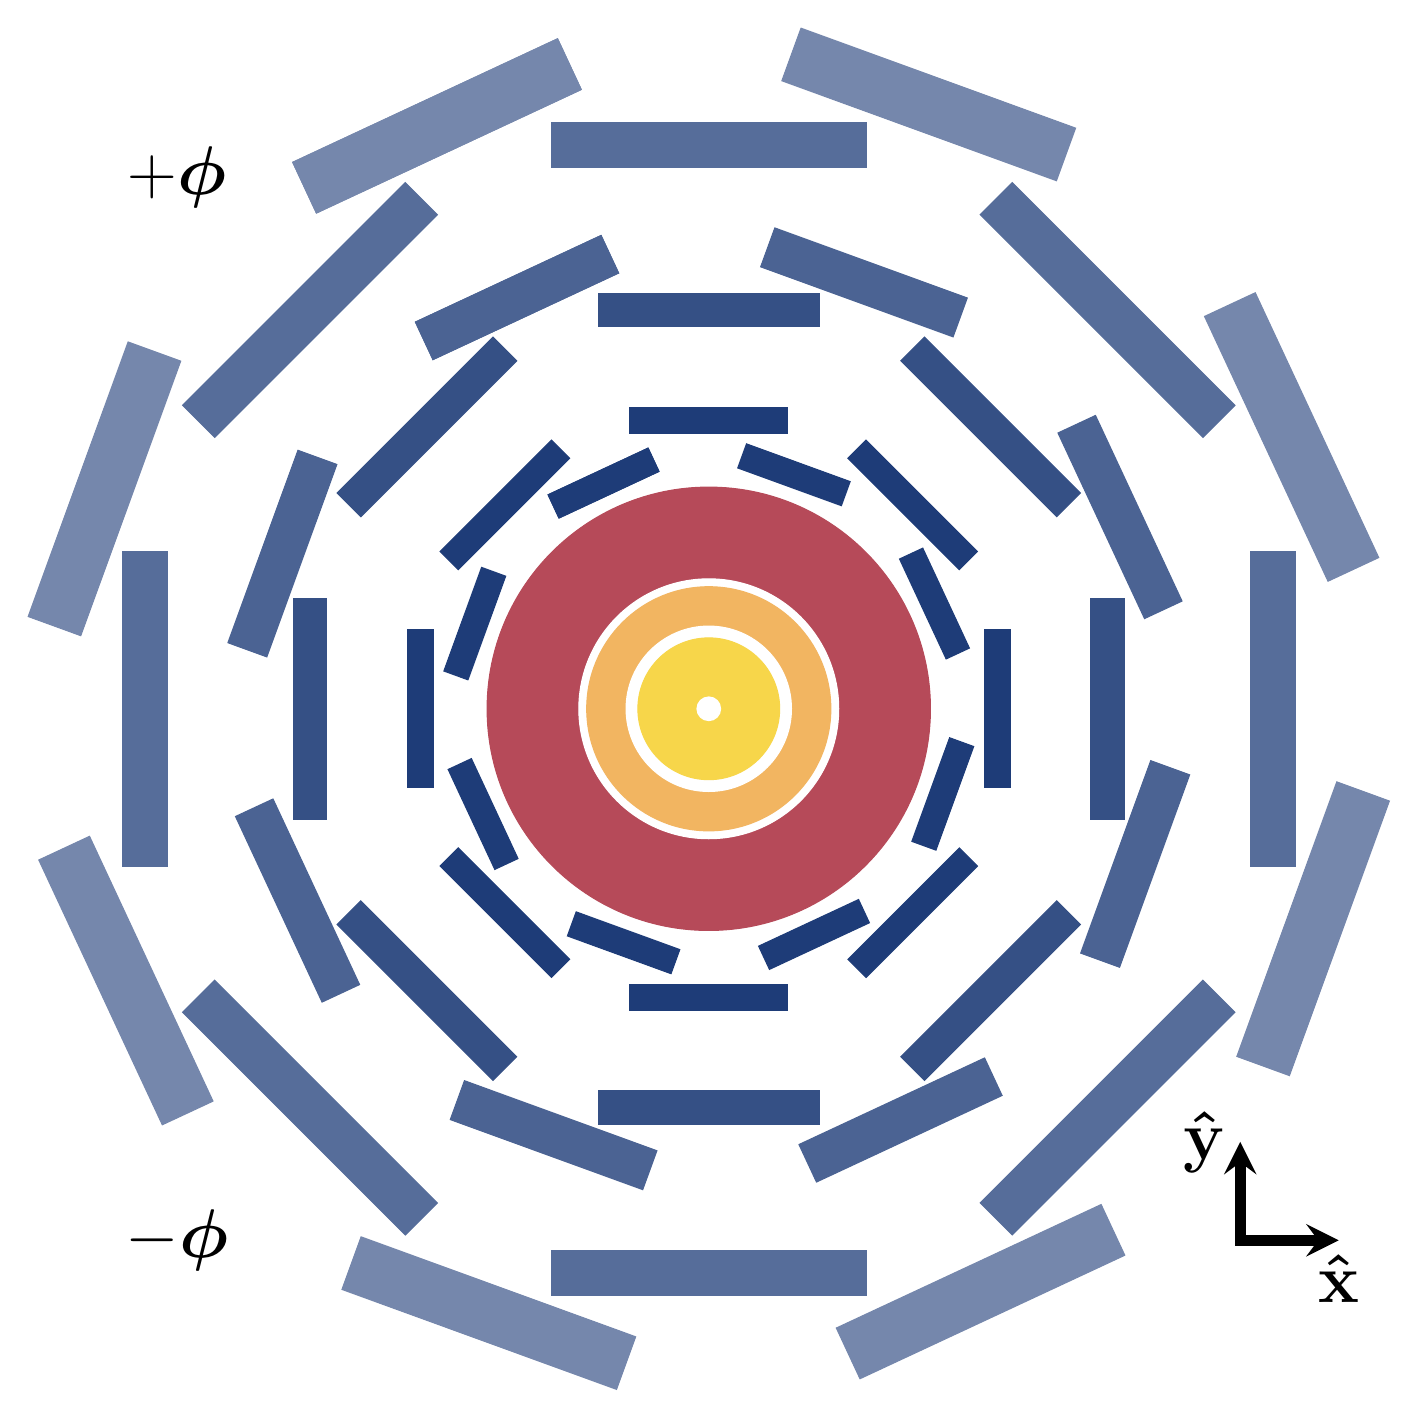
\begin{tikzpicture}[scale=0.5]
\draw[fill=outer!80, draw=outer!80] (0,0) circle (5.63); 
\draw[fill=white, draw=white] (0,0) circle (3.3);
\draw[fill=middle!80, draw=middle!80] (0,0) circle (3.1); 
\draw[fill=white, draw=white] (0,0) circle (2.1);
\draw[fill=inner, draw=inner] (0,0) circle (1.8);
\draw[fill=white!80, draw=white!80] (0,0) circle (0.3);
\foreach \y in {0, 1, 2.5}
    \foreach \a in {0, 45, 90, ..., 360}
        \pgfmathsetmacro\k{100-\y*10}
        \draw[fill=ms!\k, draw=ms!\k, rotate around={\a:(0,0)}] (-2-0.8*\y, 7 + 2.7*\y) rectangle ++(4+2*0.8*\y,0.65 + 0.2*\y);
\foreach \y in {0, 2, 3.85}
    \foreach \a in {25, 70, ..., 385}
        \pgfmathsetmacro\k{100-\y*10}
        \draw[fill=ms!\k, draw=ms!\k, rotate around={\a:(0,0)}] (-1.4-0.6*\y, 6 + 2.5*\y) rectangle ++(2.8+2*0.6*\y,0.65 + 0.2*\y);
\draw[-stealth, line width=4pt] (13.5,-13.5) -- (16,-13.5) node[below]{{\Huge $\vu{x}$}};
\draw[-stealth, line width=4pt] (13.5,-13.639) -- (13.5,-11) node[left]{{\Huge $\vu{y}$}};
\draw (-13.5,-13.5) node[]{{\Huge $-\boldsymbol{\phi}$}};
\draw (-13.5,+13.5) node[]{{\Huge $+\boldsymbol{\phi}$}};
\end{tikzpicture}

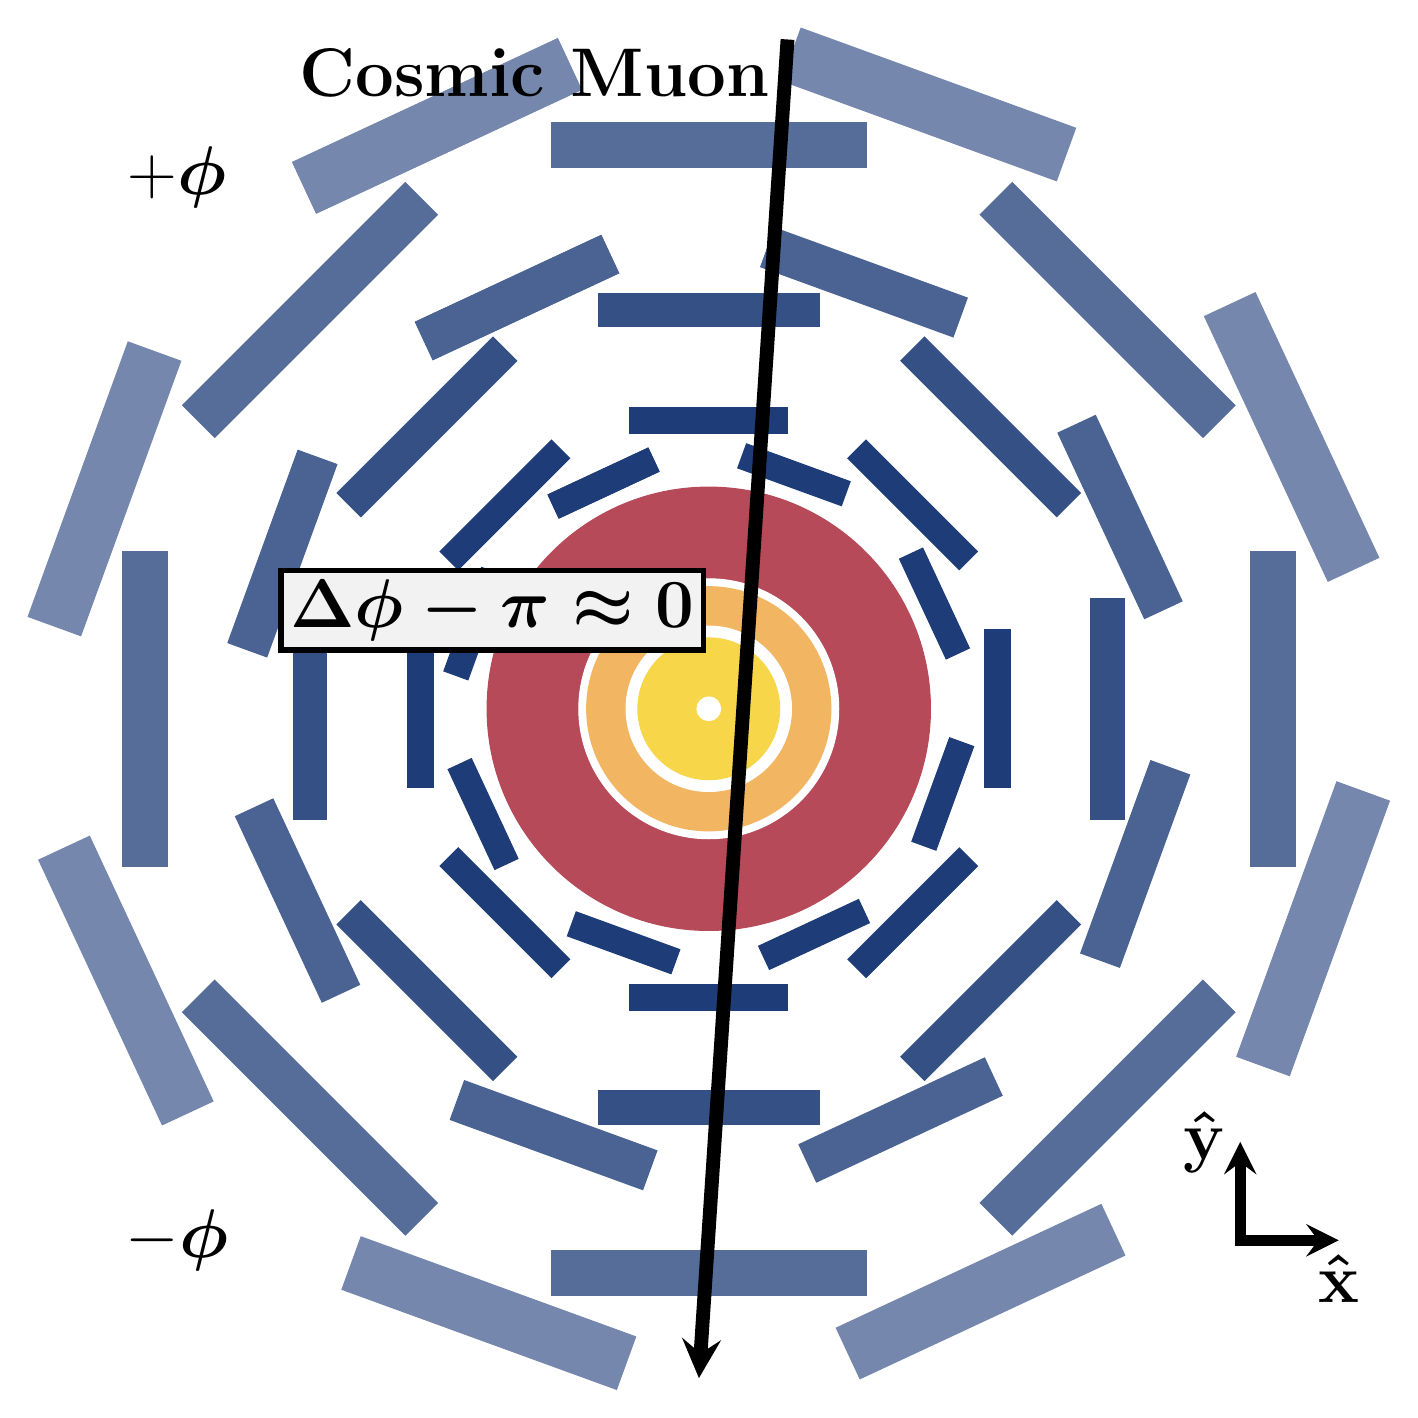
\begin{tikzpicture}[scale=0.5]
\draw[fill=outer!80, draw=outer!80] (0,0) circle (5.63); 
\draw[fill=white, draw=white] (0,0) circle (3.3);
\draw[fill=middle!80, draw=middle!80] (0,0) circle (3.1); 
\draw[fill=white, draw=white] (0,0) circle (2.1);
\draw[fill=inner, draw=inner] (0,0) circle (1.8);
\draw[fill=white!80, draw=white!80] (0,0) circle (0.3);
\foreach \y in {0, 1, 2.5}
    \foreach \a in {0, 45, 90, ..., 360}
        \pgfmathsetmacro\k{100-\y*10}
        \draw[fill=ms!\k, draw=ms!\k, rotate around={\a:(0,0)}] (-2-0.8*\y, 7 + 2.7*\y) rectangle ++(4+2*0.8*\y,0.65 + 0.2*\y);
\foreach \y in {0, 2, 3.85}
    \foreach \a in {25, 70, ..., 385}
        \pgfmathsetmacro\k{100-\y*10}
        \draw[fill=ms!\k, draw=ms!\k, rotate around={\a:(0,0)}] (-1.4-0.6*\y, 6 + 2.5*\y) rectangle ++(2.8+2*0.6*\y,0.65 + 0.2*\y);
\draw[-stealth, line width=4pt] (13.5,-13.5) -- (16,-13.5) node[below]{{\Huge $\vu{x}$}};
\draw[-stealth, line width=4pt] (13.5,-13.639) -- (13.5,-11) node[left]{{\Huge $\vu{y}$}};
\draw (-13.5,-13.5) node[]{{\Huge $-\boldsymbol{\phi}$}};
\draw (-13.5,+13.5) node[]{{\Huge $+\boldsymbol{\phi}$}};

\draw[-stealth, black, line width=5pt] (2,17) -- (-0.25,-17) node[pos=0.025,left]{\Huge \textbf{Cosmic Muon}};
\draw (-5.5,2.5) node[fill=black!5, draw = black, line width=2pt]{{\Huge $\boldsymbol{\Delta\phi-\pi\approx 0}$}};
\end{tikzpicture}

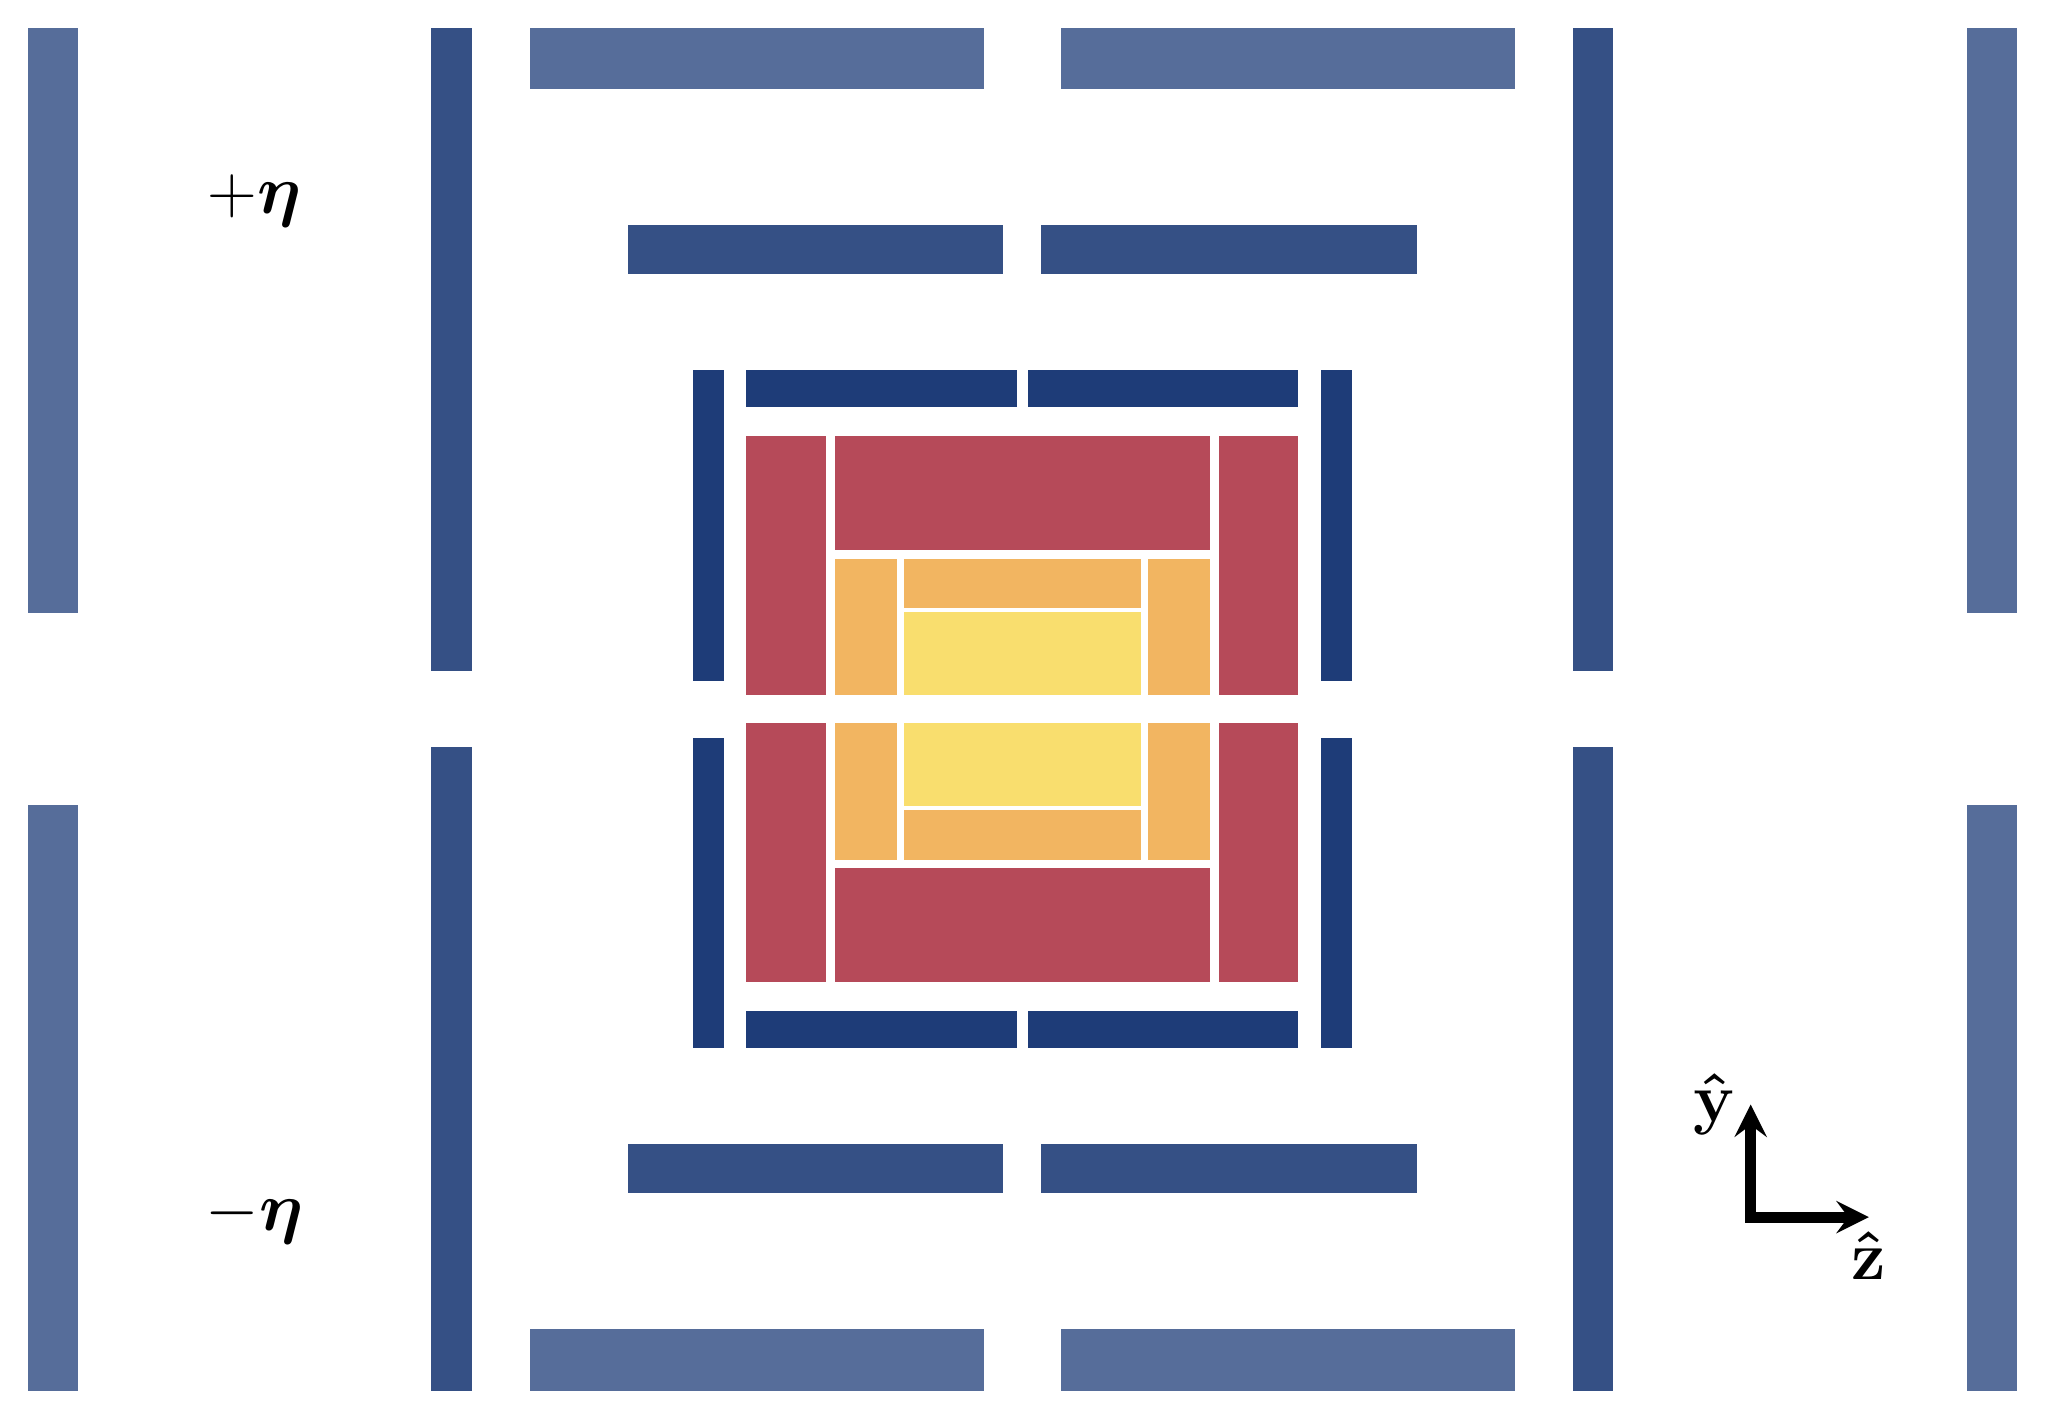
\begin{tikzpicture}[scale=0.5,yscale=1.2288]
\foreach \x in {1,-1}{
    \foreach \y in {1,-1}{
        \draw[fill=inner!80, draw=inner!80] (-3,\y*0.3) rectangle ++(2*3,\y*1.7);
        \draw[fill=middle!80, draw=middle!80] (-3,\y*2.1) rectangle ++(2*3,\y*1);
        \draw[fill=middle!80, draw=middle!80] (\x*3.2, \y*0.3) rectangle ++(\x*1.55, \y*2.8);
        \draw[fill=outer!80, draw=outer!80] (-4.75, \y*3.3) rectangle ++(2*4.75, \y*2.33);
        \draw[fill=outer!80, draw=outer!80] (\x*5, \y*0.3) rectangle ++(\x*2, \y*5.33);
        \draw[fill=ms!100, draw=ms!100] (\x*0.15, \y*6.25) rectangle ++(\x*6.85, \y*0.75);
        \draw[fill=ms!100, draw=ms!100] (\x*7.6, \y*0.6) rectangle ++(\x*0.75, \y*6.4);
        \draw[fill=ms!90, draw=ms!90] (\x*14, \y*0.8) rectangle ++(\x*1, \y*13.275);
        \draw[fill=ms!75, draw=ms!75] (\x*24, \y*2) rectangle ++(\x*1.25, \y*12.075);
        \draw[fill=ms!90, draw=ms!90] (\x*0.5, \y*9) rectangle ++(\x*9.5, \y*1);
        \draw[fill=ms!75, draw=ms!75] (\x*1, \y*12.825) rectangle ++(\x*11.5, \y*1.25);
    }
}
\draw[-stealth, line width=4pt] (18.5,-10.5) -- (21.5,-10.5) node[below]{{\Huge $\vu{z}$}};
\draw[-stealth, line width=4pt] (18.5,-10.615) -- +(0,2.4413) node[left]{{\Huge $\vu{y}$}};

\draw (-19.5,-10.5) node[]{{\Huge $-\boldsymbol{\eta}$}};
\draw (-19.5,+10.5) node[]{{\Huge $+\boldsymbol{\eta}$}};
\end{tikzpicture}

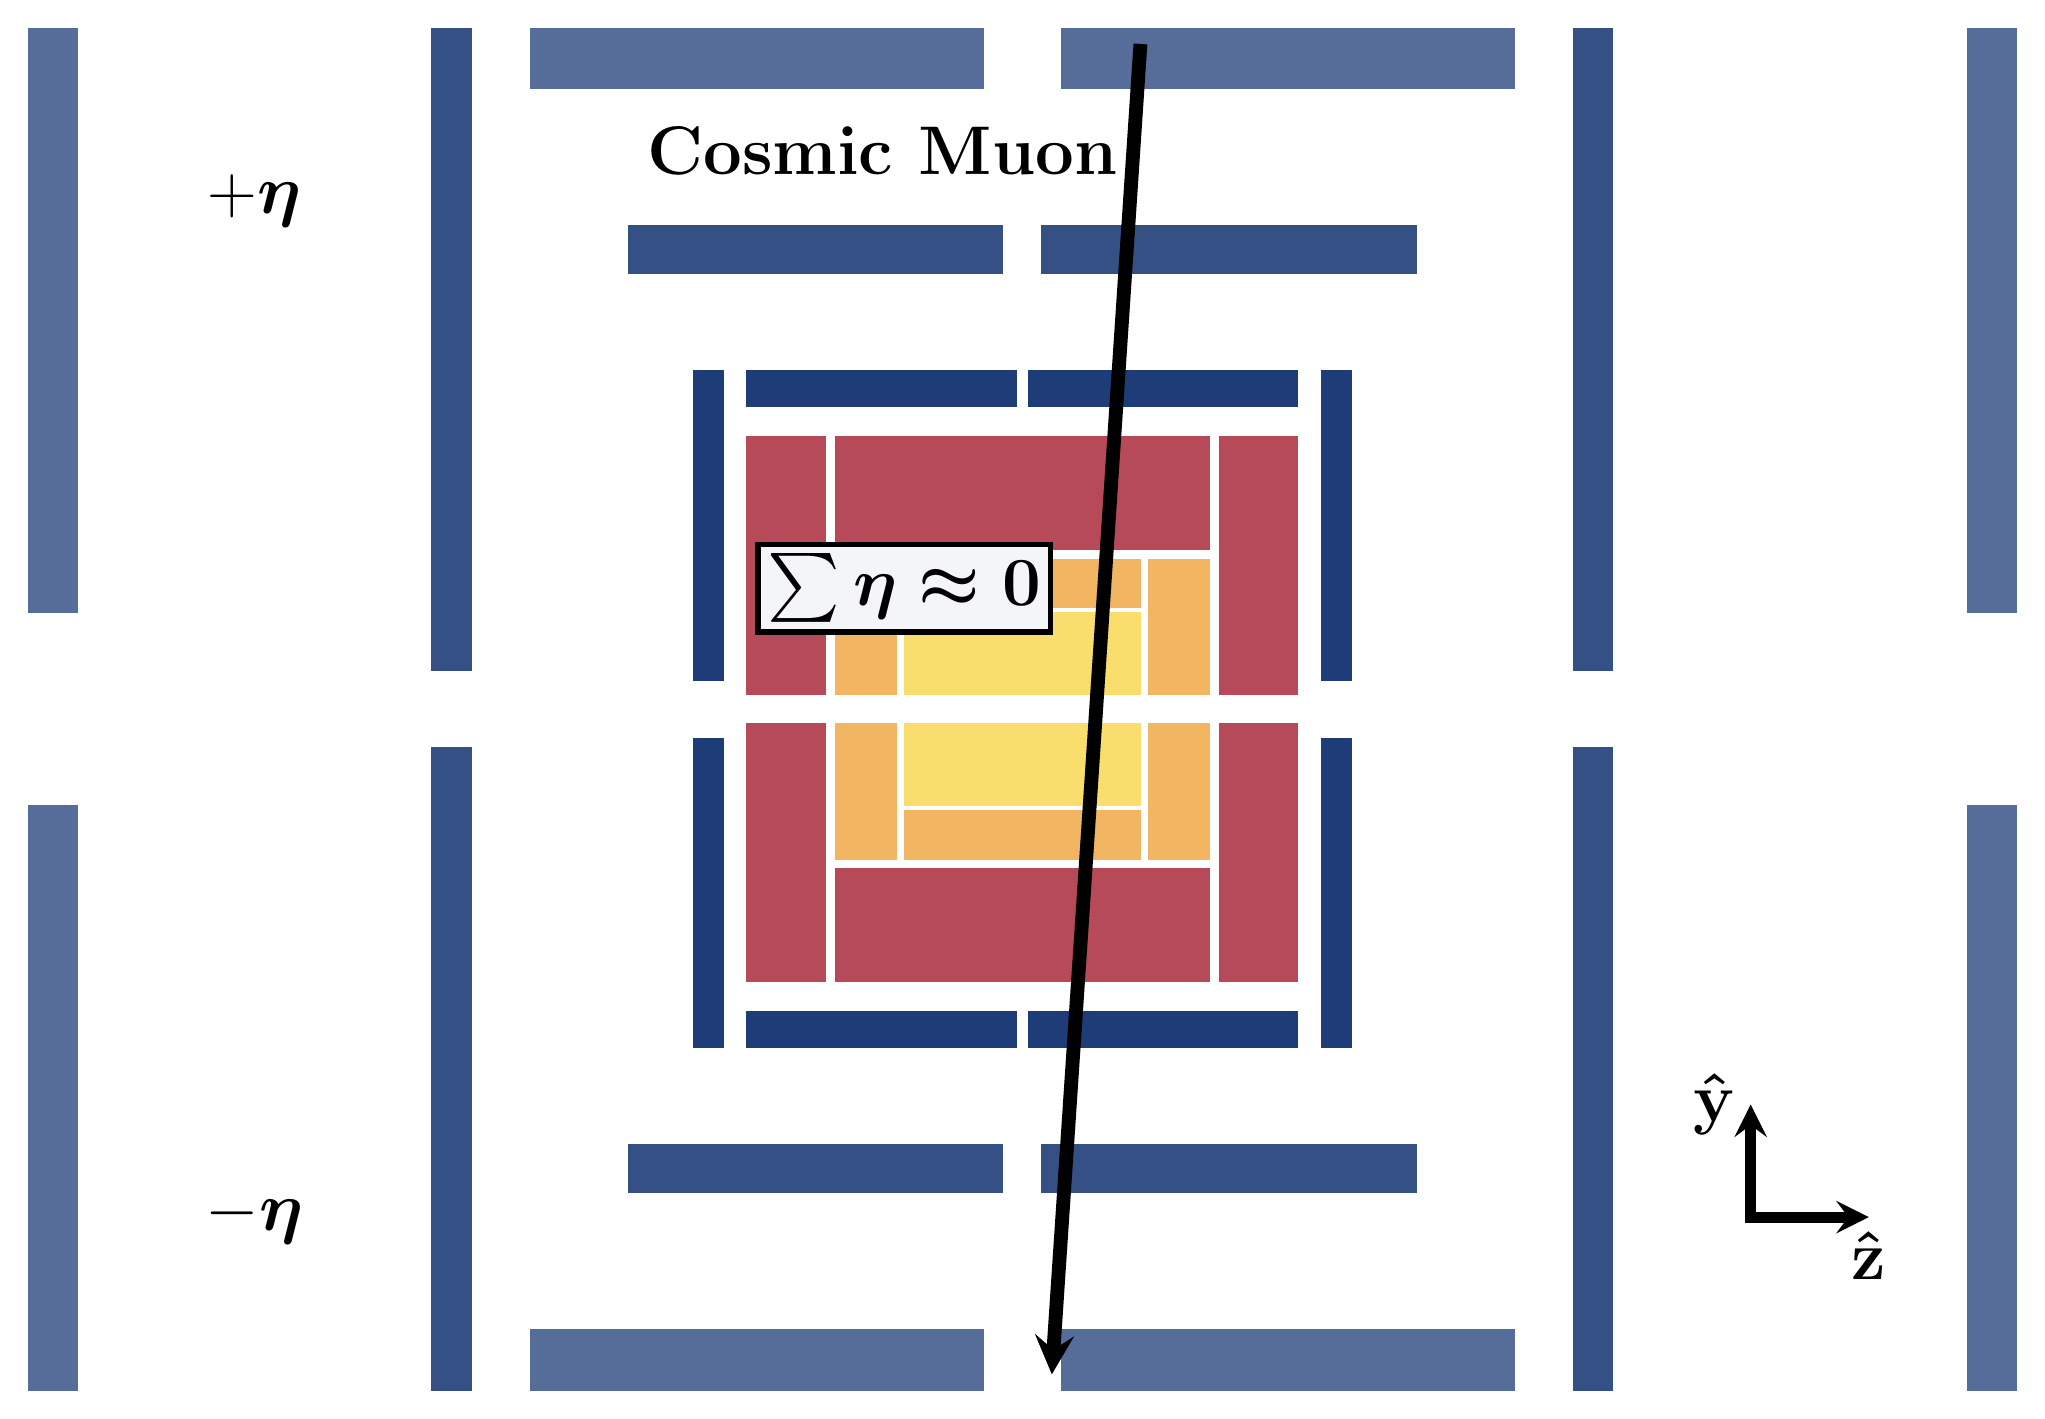
\begin{tikzpicture}[scale=0.5,yscale=1.2288]
\foreach \x in {1,-1}{
    \foreach \y in {1,-1}{
        \draw[fill=inner!80, draw=inner!80] (-3,\y*0.3) rectangle ++(2*3,\y*1.7);
        \draw[fill=middle!80, draw=middle!80] (-3,\y*2.1) rectangle ++(2*3,\y*1);
        \draw[fill=middle!80, draw=middle!80] (\x*3.2, \y*0.3) rectangle ++(\x*1.55, \y*2.8);
        \draw[fill=outer!80, draw=outer!80] (-4.75, \y*3.3) rectangle ++(2*4.75, \y*2.33);
        \draw[fill=outer!80, draw=outer!80] (\x*5, \y*0.3) rectangle ++(\x*2, \y*5.33);
        \draw[fill=ms!100, draw=ms!100] (\x*0.15, \y*6.25) rectangle ++(\x*6.85, \y*0.75);
        \draw[fill=ms!100, draw=ms!100] (\x*7.6, \y*0.6) rectangle ++(\x*0.75, \y*6.4);
        \draw[fill=ms!90, draw=ms!90] (\x*14, \y*0.8) rectangle ++(\x*1, \y*13.275);
        \draw[fill=ms!75, draw=ms!75] (\x*24, \y*2) rectangle ++(\x*1.25, \y*12.075);
        \draw[fill=ms!90, draw=ms!90] (\x*0.5, \y*9) rectangle ++(\x*9.5, \y*1);
        \draw[fill=ms!75, draw=ms!75] (\x*1, \y*12.825) rectangle ++(\x*11.5, \y*1.25);
    }
}
\draw[-stealth, line width=4pt] (18.5,-10.5) -- (21.5,-10.5) node[below]{{\Huge $\vu{z}$}};
\draw[-stealth, line width=4pt] (18.5,-10.615) -- +(0,2.4413) node[left]{{\Huge $\vu{y}$}};

\draw (-19.5,-10.5) node[]{{\Huge $-\boldsymbol{\eta}$}};
\draw (-19.5,+10.5) node[]{{\Huge $+\boldsymbol{\eta}$}};

\draw[-stealth, black, line width=5pt] (3,13.75) -- (0.75,-13.75) node[pos=0.08,left]{\Huge \textbf{Cosmic Muon}};
\draw (-3,2.5) node[fill=ms!5, draw = black, line width=2pt]{{\Huge $\boldsymbol{\sum\eta\approx 0}$}};
\end{tikzpicture}


\end{document}